For the feedback transresistance amplifier in \ref{fig:ee18btech11046_Question}), use small-signal analysis to find the open-loop gain 'G', Feedback factor 'H' and Closed-loop gain 'T'. Let $R_{F}>>R_{L}$ and $r_{o}>>R_{L}$. Find the value of T for $R_{L}=10K\ohm$, $R_{F}=100K\ohm$ and the transistor current gain $\beta = 100$.
\begin{enumerate}[label=\thesection.\arabic*.,ref=\thesection.\theenumi]
\numberwithin{equation}{enumi}    
\item Draw the equivalent control system for the feedback Transresistance amplifier shown in \ref{fig:ee18btech11046_Question}
\renewcommand{\thefigure}{\theenumi.\arabic{figure}}
\begin{figure}[h!]
	\begin{center}
		\resizebox{\columnwidth/1}{!}{
\begin{circuitikz}[american,node distance = 30pt]
\draw (0,0) node[npn](npn1) {}
  (npn1.base) node[anchor=east,yshift=-0.25cm] {B}
  (npn1.collector) node[anchor=south,xshift=0.25cm,yshift=-0.25cm] {C}
  (npn1.emitter) node[anchor=north,xshift=0.25cm] {E};
\draw (npn1.collector) to[R,l_=$R_L$] ++(0,3) to [short,-o]++(0,0.5) node[right]{$V_{cc}$};
\draw (npn1.emitter) to[short] node[ground]{GND}++(0,-2);
\draw (npn1.base) to[short,i<=$I_i$] ++(-3,0) to [I,invert,l_=$I_s$] ++(0,-2) node[ground]{};
\draw (npn1.base) -- ++(-2,0) to [short,*-]++(0,1) to [short,i=$I_F$]++(1,0) to [R,l=$R_F$]++(1,0) to [short,-*]++(0.85,0) to [short,-o]++(0.85,0) node[right]{$V_o$};

\end{circuitikz}
}
	\end{center}
	\caption{}
	\label{fig:ee18btech11046_Question}
\end{figure}
\\

%
\solution see Fig. \ref{fig:ee18btech11046_ControlSystem}
\begin{figure}[ht!]
	\begin{center}
		\resizebox{\columnwidth}{!}{\tikzstyle{block} = [draw, rectangle, 
    minimum height=1.25em, minimum width=2.5em]
\tikzstyle{sum} = [draw, circle, node distance=1cm]
\tikzstyle{input} = [coordinate]
\tikzstyle{output} = [coordinate]
\tikzstyle{pinstyle} = [pin edge={to-,thin,black}]

% The block diagram code is probably more verbose than necessary
\begin{tikzpicture}[auto, node distance=2.5cm,>=latex']
    % We start by placing the blocks
    \node [input, name=input] {};
    \node [sum, right of=input] (sum) {};
    \node [block, right of=sum] (controller) {$G$};
    
    % We draw an edge between the controller and system block to 
    % calculate the coordinate u. We need it to place the measurement block. 
   
    \node [output, right of=controller] (output) {};
    \node [block, below of=controller] (measurements) {$H$};

    % Once the nodes are placed, connecting them is easy. 
    \draw [draw,->] (input) -- node[pos=0.99] {$+$} node {$I_{s}$} (sum);
    \draw [->] (sum) -- node {$I_{i}$} (controller);
    \draw [->] (controller) -- node [name=y] {$v_{o}$}(output);
    \draw [->] (y) |- (measurements);
    \draw [->] (measurements) -| node[pos=0.99] {$-$} node [near end] {$I_{F}$} (sum);
\end{tikzpicture}
}
	\end{center}
	\caption{}
	\label{fig:ee18btech11046_ControlSystem}
\end{figure}
\renewcommand{\thefigure}{\theenumi}

%

\item For the feedback Transresistance amplifier shown in \ref{fig:ee18btech11046_Question}, Draw its small signal model. Early effect in Transistor is neglected.
\\

%
\solution see Fig. \ref {fig:ee18btech11046_smallSig}

While drawing a Small-Signal Model, we
ground all constant voltage sources and open
all constant current sources. All Small-Signal
paramters are obtained from DC-Analysis of
the circuit. Neglecting Early effect, in SmallSignal Analysis a npn-Transistor is modelled as
a Current Source with value of current equal to
$g_{m}V_{be}$ flowing from Collextor to Emitter. Whereas
a pnp-Transistor is modelled as a Current Source
with value of current equal to $g_{m}V_{be}$ flowing
from Emitter to Collector.

\begin{figure}[ht!]
	\begin{center}
		\resizebox{\columnwidth}{!}{
\begin{circuitikz}[american,node distance = 30pt]
\draw (0,0) node[ground]{};
\draw (0,0) to [I,l=$I_{s}$]++(0,2);
\draw (0,2) to [short]++(1,0) to [short,i=$I_{i}$]++(1,0);
\draw (2,2) to [R,v=$v_{be}$,l=$r_{\pi}$] ++(0,-2) to [short]++(3,0) to[I,invert,l=$g_{m}$$v_{be}$]++(0,2);
\draw (5,2) to [short]++(2,0) to [R,i=$I_{o}$,l=$R_{L}$]++(0,-2);
\draw (7,2) to [short,-o]++(2,0) node[right]{$V_{o}$};
\draw (1,2) to [short,i = $I_{F}$,*-]++(0,1) to [R,l=$R_{F}$]++(6,0) to [short,-*]++(0,-1);
\draw (3.5,0) node[ground]{};
\draw (7,0) node[ground]{};
\end{circuitikz}
}
	\end{center}
	\caption{Small Signal Model}
	\label{fig:ee18btech11046_smallSig}
\end{figure}
\renewcommand{\thefigure}{\theenumi}

%


\item Find small signal parameters 
 $g_{m}$ and $v_{be}$ using DC analysis
\\
%
\solution
small signal parameters of bjt are given in
\eqref{eq:ee18btech11046_gm} and \eqref{eq:ee18btech11046_rpi}
\begin{align}
g_{m} = \frac{I_{C}}{V_{T}}
\label{eq:ee18btech11046_gm}
\end{align}
\begin{align}
r_{\pi} = \frac{V_{T}}{I_{B}}
\label{eq:ee18btech11046_rpi}
\end{align}
The Large signal model of circuit becomes as shown in figure \ref{fig:ee18btech11046_largeSig}
\begin{figure}[ht!]
	\begin{center}
		\resizebox{\columnwidth}{!}{
\begin{circuitikz}[american,node distance = 30pt]
\draw (0,0) node[npn](npn1) {}
  (npn1.base) node[anchor=east,yshift=-0.25cm] {B}
  (npn1.collector) node[anchor=south,xshift=0.25cm,yshift=-0.25cm] {C}
  (npn1.emitter) node[anchor=north,xshift=0.25cm] {E};
\draw (npn1.collector)to [short,i<=$I_c$]++(0,0.5) to[R,l_=$R_L$,i<=$I_E$] ++(0,3) to [short,-o]++(0,0.5) node[right]{$V_{cc}$};
\draw (npn1.emitter) to[short,i=$I_E$] node[ground]{GND}++(0,-2);
\draw (npn1.base) -- ++(-2,0) to [short]++(0,1.5) to [short,i<=$I_B$]++(1,0) to [R,l=$R_F$]++(1,0) to [short]++(0.85,0);

\end{circuitikz}
}
	\end{center}
	\caption{Large signal model}
	\label{fig:ee18btech11046_largeSig}
\end{figure}
\renewcommand{\thefigure}{\theenumi}


Where $V_{T} = 25m$volts
\begin{align}
V_{BE} = 0.7 volts 
\implies
V_{B} = 0.7 volts
\end{align}

\begin{align}
I_{E} = I_{B} + I_{C}
\end{align}
\begin{align}
I_{C} = \beta I_{B}
\end{align}

From applying KVL and KCL on Fig.
\begin{align}
V_{cc} - I_{E}R_{L} - I_{B}R_{F} - 0.7 = 0
\\
\implies
V_{cc} - \brak{\beta+1}I_{B}R_{L} - I_{B}R_{F} - 0.7 = 0
\end{align}
\begin{align}
I_{B} = \frac{V_{cc}-0.7}{\brak{\beta+1}R_{L}+R_{F}}
\label{eq:ee18btech11046_IB}
\end{align}
\begin{align}
I_{C} = \beta \frac{V_{cc}-0.7}{\brak{\beta+1}R_{L}+R_{F}}
\label{eq:ee18btech11046_IC}
\end{align}
from \eqref{eq:ee18btech11046_gm}, \eqref{eq:ee18btech11046_rpi},$I_{B}$ and $I_{C}$
\begin{align}
g_{m} = \frac{\beta}{V_{T}}\frac{V_{cc}-0.7}{\brak{\beta+1}R_{L}+R_{F}}
\label{eq:ee18btech11046_gmval}
\end{align}

\begin{align}
r_{\pi} = V_{T}\frac{\brak{\beta+1}R_{L}+R_{F}}{V_{cc}-0.7}
\label{eq:ee18btech11046_rpival}
\end{align}

%

\item Write all node/loop equations of Small-Signal model using KCL/KVL.Given that $R_{F} >> R_{L}$\\
%
\solution
\begin{align}
v_{be} = I_{i}r_{\pi}
\label{eq:ee18btech11046_eq1}
\end{align}
\begin{align}
v_{be} - I_{F}R_{F} = V_{o}
\label{eq:ee18btech11046_eq2}
\end{align}
\begin{align}
V_{o} = \brak{I_{F} - g_{m}v_{be}}R_{L}
\label{eq:ee18btech11046_eq3}
\end{align}
%

\item Find the expression for feedback factor H.\\
%
\solution
\begin{align}
H = \frac{I_{F}}{V_{o}}
\end{align}
substituting \eqref{eq:ee18btech11046_eq2} in \eqref{eq:ee18btech11046_eq3}
\begin{align}
V_{o} = \brak{I_{F}-g_{m}V_{o}-g_{m}I_{F}R_{F}}R_{L}
\\
\implies
\brak{1+g_{m}R_{L}}V_{o} = I_{F}\brak{R_{L}-g_{m}R_{F}R_{L}}
\end{align}
\begin{align}
H = \frac{I_{F}}{V_{o}} = \frac{1+g_{m}R_{L}}{R_{L}\brak{1-g_{m}R_{F}}}
\label{eq:ee18btech11046_H}
\\
\implies H \approx -\frac{1}{R_{F}}
\label{eq:ee18btech11046_Happrox}
\end{align}
%

\item Find the expression for Open loop Gain G.\\
%
\solution
\begin{align}
G = \frac{V_{o}}{I_{i}}
\end{align}
 Substituting \eqref{eq:ee18btech11046_eq1} in \eqref{eq:ee18btech11046_eq2} and subistituting $I_{F}$ from
\eqref{eq:ee18btech11046_H}
\begin{align}
I_{i}r_{\pi} -\brak{\frac{1+g_{m}R_{L}}{R_{L}\brak{1-1+g_{m}R_{F}}}}R_{F}V_{o} = V_{o}
\\
\implies
G = \frac{V_{o}}{I_{i}} = \frac{r_{\pi}R_{L}\brak{1-g_{m}R_{F}}}{R_{F}+R_{L}}
\label{eq:ee18btech11046_G}
\end{align}
Upon approximating since $R_{F} >> R_{L}$
\begin{align}
G = -g_{m}r_{\pi}R_{L}
\label{eq:ee18btech11046_Gapprox}
\end{align}

%
\item Find the expression for Closed Loop Gain $T = \frac{V_{o}}{I_{s}}$
%
We know that Closed Loop Gain
\begin{align}
T = \frac{G}{1+GH}
\end{align}
Substituting expressions from \eqref{eq:ee18btech11046_Happrox} and \eqref{eq:ee18btech11046_G}
\begin{align}
T = -\frac{g_{m}r_{\pi}R_{L}}{1+\brak{\frac{g_{m}r_{\pi}R_{L}}{R_{F}}}}
\label{eq:ee18btech11046_T}
\end{align}
%

\item For the parameters given in table \ref{table:ee18btech11046_Table_1} . Find G,H and T.
%
\begin{table}[!ht]
\centering


%%  This section checks if we are begin input into another file or  %%
%%  the file will be compiled alone. First use a macro taken from   %%
%%  the TeXbook ex 7.7 (suggestion of Han-Wen Nienhuys).            %%
\def\ifundefined#1{\expandafter\ifx\csname#1\endcsname\relax}


%%  Check for the \def token for inputed files. If it is not        %%
%%  defined, the file will be processed as a standalone and the     %%
%%  preamble will be used.                                          %%
\ifundefined{inputGnumericTable}

%%  We must be able to close or not the document at the end.        %%
	\def\gnumericTableEnd{\end{document}}


%%%%%%%%%%%%%%%%%%%%%%%%%%%%%%%%%%%%%%%%%%%%%%%%%%%%%%%%%%%%%%%%%%%%%%
%%                                                                  %%
%%  This is the PREAMBLE. Change these values to get the right      %%
%%  paper size and other niceties.                                  %%
%%                                                                  %%
%%%%%%%%%%%%%%%%%%%%%%%%%%%%%%%%%%%%%%%%%%%%%%%%%%%%%%%%%%%%%%%%%%%%%%

	\documentclass[12pt%
			  %,landscape%
                    ]{report}
       \usepackage[latin1]{inputenc}
       \usepackage{fullpage}
       \usepackage{color}
       \usepackage{array}
       \usepackage{longtable}
       \usepackage{calc}
       \usepackage{multirow}
       \usepackage{hhline}
       \usepackage{ifthen}
%%  End of the preamble for the standalone. The next section is for %%
%%  documents which are included into other LaTeX2e files.          %%
\else

%%  We are not a stand alone document. For a regular table, we will %%
%%  have no preamble and only define the closing to mean nothing.   %%
    \def\gnumericTableEnd{}

%%  If we want landscape mode in an embedded document, comment out  %%
%%  the line above and uncomment the two below. The table will      %%
%%  begin on a new page and run in landscape mode.                  %%
%       \def\gnumericTableEnd{\end{landscape}}
%       \begin{landscape}


%%  End of the else clause for this file being \input.              %%
\fi

%%%%%%%%%%%%%%%%%%%%%%%%%%%%%%%%%%%%%%%%%%%%%%%%%%%%%%%%%%%%%%%%%%%%%%
%%                                                                  %%
%%  The rest is the gnumeric table, except for the closing          %%
%%  statement. Changes below will alter the table's appearance.     %%
%%                                                                  %%
%%%%%%%%%%%%%%%%%%%%%%%%%%%%%%%%%%%%%%%%%%%%%%%%%%%%%%%%%%%%%%%%%%%%%%

\providecommand{\gnumericmathit}[1]{#1} 
%%  Uncomment the next line if you would like your numbers to be in %%
%%  italics if they are italizised in the gnumeric table.           %%
%\renewcommand{\gnumericmathit}[1]{\mathit{#1}}
\providecommand{\gnumericPB}[1]%
{\let\gnumericTemp=\\#1\let\\=\gnumericTemp\hspace{0pt}}
 \ifundefined{gnumericTableWidthDefined}
        \newlength{\gnumericTableWidth}
        \newlength{\gnumericTableWidthComplete}
        \newlength{\gnumericMultiRowLength}
        \global\def\gnumericTableWidthDefined{}
 \fi
%% The following setting protects this code from babel shorthands.  %%
 \ifthenelse{\isundefined{\languageshorthands}}{}{\languageshorthands{english}}
%%  The default table format retains the relative column widths of  %%
%%  gnumeric. They can easily be changed to c, r or l. In that case %%
%%  you may want to comment out the next line and uncomment the one %%
%%  thereafter                                                      %%
\providecommand\gnumbox{\makebox[0pt]}
%%\providecommand\gnumbox[1][]{\makebox}

%% to adjust positions in multirow situations                       %%
\setlength{\bigstrutjot}{\jot}
\setlength{\extrarowheight}{\doublerulesep}

%%  The \setlongtables command keeps column widths the same across  %%
%%  pages. Simply comment out next line for varying column widths.  %%
\setlongtables

\setlength\gnumericTableWidth{%
	60pt+%
	100pt+%
0pt}
\def\gumericNumCols{2}
\setlength\gnumericTableWidthComplete{\gnumericTableWidth+%
         \tabcolsep*\gumericNumCols*2+\arrayrulewidth*\gumericNumCols}
\ifthenelse{\lengthtest{\gnumericTableWidthComplete > \linewidth}}%
         {\def\gnumericScale{\ratio{\linewidth-%
                        \tabcolsep*\gumericNumCols*2-%
                        \arrayrulewidth*\gumericNumCols}%
{\gnumericTableWidth}}}%
{\def\gnumericScale{1}}

%%%%%%%%%%%%%%%%%%%%%%%%%%%%%%%%%%%%%%%%%%%%%%%%%%%%%%%%%%%%%%%%%%%%%%
%%                                                                  %%
%% The following are the widths of the various columns. We are      %%
%% defining them here because then they are easier to change.       %%
%% Depending on the cell formats we may use them more than once.    %%
%%                                                                  %%
%%%%%%%%%%%%%%%%%%%%%%%%%%%%%%%%%%%%%%%%%%%%%%%%%%%%%%%%%%%%%%%%%%%%%%

\ifthenelse{\isundefined{\gnumericColA}}{\newlength{\gnumericColA}}{}\settowidth{\gnumericColA}{\begin{tabular}{@{}p{60pt*\gnumericScale}@{}}x\end{tabular}}
\ifthenelse{\isundefined{\gnumericColB}}{\newlength{\gnumericColB}}{}\settowidth{\gnumericColB}{\begin{tabular}{@{}p{100pt*\gnumericScale}@{}}x\end{tabular}}
\begin{tabular}[c]{%
	b{\gnumericColA}%
	b{\gnumericColB}%%
	}

%%%%%%%%%%%%%%%%%%%%%%%%%%%%%%%%%%%%%%%%%%%%%%%%%%%%%%%%%%%%%%%%%%%%%%
%%  The longtable options. (Caption, headers... see Goosens, p.124) %%
%	\caption{The Table Caption.}             \\	%
% \hline	% Across the top of the table.
%%  The rest of these options are table rows which are placed on    %%
%%  the first, last or every page. Use \multicolumn if you want.    %%

%%  Header for the first page.                                      %%
%	\multicolumn{3}{c}{The First Header} \\ \hline 
%	\multicolumn{1}{c}{colTag}	%Column 1
%	&\multicolumn{1}{c}{colTag}	%Column 2
%	&\multicolumn{1}{c}{colTag}	\\ \hline %Last column
%	\endfirsthead

%%  The running header definition.                                  %%
%	\hline
%	\multicolumn{3}{l}{\ldots\small\slshape continued} \\ \hline
%	\multicolumn{1}{c}{colTag}	%Column 1
%	&\multicolumn{1}{c}{colTag}	%Column 2
%	&\multicolumn{1}{c}{colTag}	\\ \hline %Last column
%	\endhead

%%  The running footer definition.                                  %%
%	\hline
%	\multicolumn{3}{r}{\small\slshape continued\ldots} \\
%	\endfoot

%%  The ending footer definition.                                   %%
%	\multicolumn{3}{c}{That's all folks} \\ \hline 
%	\endlastfoot
%%%%%%%%%%%%%%%%%%%%%%%%%%%%%%%%%%%%%%%%%%%%%%%%%%%%%%%%%%%%%%%%%%%%%%

\hhline{|-|-}
	 \multicolumn{1}{|p{\gnumericColA}|}%
	{\gnumericPB{\centering}\textbf{Parameters}}
	&\multicolumn{1}{p{\gnumericColB}|}%
	{\gnumericPB{\centering}\textbf{Value}}

	
\\
\hhline{|--|}
	 \multicolumn{1}{|p{\gnumericColA}|}%
	{\gnumericPB{\centering}$V_{cc}$}
	&\multicolumn{1}{p{\gnumericColB}|}%
	{\gnumericPB{\centering}5V}


\\

\hhline{|--|}
	 \multicolumn{1}{|p{\gnumericColA}|}%
	{\gnumericPB{\centering}$I_{s}$}
	&\multicolumn{1}{p{\gnumericColB}|}%
	{\gnumericPB{\centering}$1\mu$A}


\\
\hhline{|--|}
	 \multicolumn{1}{|p{\gnumericColA}|}%
	{\gnumericPB{\centering}$R_{F}$}
	&\multicolumn{1}{p{\gnumericColB}|}%
	{\gnumericPB{\centering}$100K\ohm$}


\\


\hhline{|--|}
	 \multicolumn{1}{|p{\gnumericColA}|}%
	{\gnumericPB{\centering}$R_{L}$}
	&\multicolumn{1}{p{\gnumericColB}|}%
	{\gnumericPB{\centering}$10K\ohm$}


\\

\hhline{|--|}
	 \multicolumn{1}{|p{\gnumericColA}|}%
	{\gnumericPB{\centering}$\beta$}
	&\multicolumn{1}{p{\gnumericColB}|}%
	{\gnumericPB{\centering}$100$}



\\
\hhline{|-|-|}
\end{tabular}

\ifthenelse{\isundefined{\languageshorthands}}{}{\languageshorthands{\languagename}}
\gnumericTableEnd

\caption{}
\label{table:ee18btech11046_Table_1}
\end{table}
%
\solution
Substituting the parameters in \eqref{eq:ee18btech11046_gmval} and \eqref{eq:ee18btech11046_rpival} gives,
\begin{align}
r_{\pi} = 6.6667\times 10^{3} \ohm
\\
g_{m} = 0.015 S 
\end{align}
Substituting $g_{m}$, $r_{\pi}$ obtained in 
\eqref{eq:ee18btech11046_Happrox}
\begin{align}
H = -10^{-5}
\end{align}
Substituting $g_{m}$, $r_{\pi}$ obtained in 
\eqref{eq:ee18btech11046_Gapprox}
\begin{align}
G = -10^{6}
\end{align}
Substituting $g_{m}$, $r_{\pi}$ obtained in 
\eqref{eq:ee18btech11046_T}
\begin{align}
T = -90909.09
\end{align}

\item Draw the block diagram and circuit diagram for H.
\\
\solution see figs \ref{fig:ee18btech11046_Hblock}  and \ref{fig:ee18btech11046_fc}
%
\renewcommand{\thefigure}{\theenumi.\arabic{figure}}

\begin{figure}[ht!]
	\begin{center}
		\resizebox{\columnwidth}{!}{
\begin{circuitikz}[american]
\usetikzlibrary{positioning, fit, calc}
\draw (0,0) to [I,i=$I_{F}$]++(0,2)to[short]++(6,0);
\draw (0,0) to [short]++(6,0);
\draw (8,1)node[draw,minimum width=4cm,minimum height=4cm] (load) {H}(8,0)
(10,0)--++(6,0)
(10,2)--(16,2)
node at (16,1.7) {$+$}
node at (16,0.3){$-$}
node at (16,1){$V_o$}
;
\end{circuitikz}
}
	\end{center}
	\caption{Feedback block diagram}
	\label{fig:ee18btech11046_Hblock}
\end{figure}

%
%
\begin{figure}[ht!]
	\begin{center}
		\resizebox{\columnwidth}{!}{
\begin{circuitikz}[american,node distance = 30pt]
\draw (0,0) to [short,i=$I_{F}$] ++(0,2) to [R,l=$R_{F}$]++(4,0) ;
\draw (4,2) to [V,v<=$V_{o}$]++(0,-2) to [short]++(-4,0);
\draw (2,0) to [short,*-]++(0,-0.5);
\draw (2,-0.5) node[ground]{};
\end{circuitikz}
}
	\end{center}
	\caption{Feedback circuit}
	\label{fig:ee18btech11046_fc}
\end{figure}
\renewcommand{\thefigure}{\theenumi}
%

From KVl on \ref{fig:ee18btech11046_fc} we can see that
\begin{align}
H=\frac{I_{F}}{V_{o}} = -\frac{1}{R_{F}}
\end{align}

\item Find the input and output resistances of the feedback network.\\
\solution
From the feedback amplifier circuit fig.\ref{fig:ee18btech11046_fc}
To find the input resistance $R_{11}$ short
the output node $V_{o}$ to ground.
\begin{align}
R_{11} = R_{F}
\end{align}
To find the output resistance $R_{22}$ rempve the current source and short input terminals.
\begin{align}
R_{22} = R_{F}
\end{align}

\item Draw the block diagram and circuit diagram for G.
\\
\solution see figs \ref{fig:ee18btech11046_Gblock} and \ref{fig:ee18btech11046_Gcir}
%
\renewcommand{\thefigure}{\theenumi.\arabic{figure}}

\begin{figure}[ht!]
	\begin{center}
		\resizebox{\columnwidth}{!}{
\begin{circuitikz}[american]
\usetikzlibrary{positioning, fit, calc}
\draw (0,0) to [I,i=$I_{i}$]++(0,2)to[short]++(6,0);
\draw (0,0) to [short]++(6,0);
\draw (8,1)node[draw,minimum width=4cm,minimum height=4cm] (load) {G}(8,0)
(10,0)--++(6,0)
(10,2)--(16,2)
node at (16,1.7) {$+$}
node at (16,0.3){$-$}
node at (16,1){$V_o$}
;
\draw (2,0) to [R,l=$R_{s}$]++(0,2);
\draw (14,0) to [R,l=$R_{L}$]++(0,2);
\draw (4,0) to [R,l=$R_{11}$]++(0,2);
\draw (12,0) to [R,l=$R_{22}$]++(0,2);
\end{circuitikz}
}
	\end{center}
	\caption{Open loop block diagram}
	\label{fig:ee18btech11046_Gblock}
\end{figure}

%
\begin{figure}[ht!]
	\begin{center}
		\resizebox{\columnwidth}{!}{
\begin{circuitikz}[american,node distance = 30pt]
\draw (0,0) node[ground]{};
\draw (0,0) to [I,l=$I_{s}$]++(0,2);
\draw (0,2) to [short]++(1,0) to [short,i=$I_{i}$]++(1,0);
\draw (2,2) to [R,v=$v_{be}$,l=$r_{\pi}$] ++(0,-2) to [short]++(3,0) to[I,invert,l=$g_{m}$$v_{be}$]++(0,2);
\draw (5,2) to [short]++(2,0) to [R,i=$I_{o}$,l=$R_{L}$]++(0,-2);
\draw (7,2) to [short,-o]++(2,0) node[right]{$V_{o}$};
\draw (3.5,0) node[ground]{};
\draw (7,0) node[ground]{};
\end{circuitikz}
}
	\end{center}
	\caption{Open loop block circuit diagram}
	\label{fig:ee18btech11046_Gcir}
\end{figure}

\item Find G
\\
\solution
From fig.\ref{fig:ee18btech11046_Gcir},
\begin{align}
V_{be} = I_{i}r_{\pi}
\end{align}
From KCL at node $V_{o}$,
\begin{align}
I_{o} = -g_{m}I_{i}r_{\pi}
\end{align}
\begin{align}
V_{o} = -g_{m}I_{i}r_{\pi}R_{L}
\end{align}
Therefore,
\begin{align}
G =\frac{V_{o}}{I_{i}} = -g_{m}r_{\pi}R_{L}
\end{align}

\item Simulate the circuit using ngspice
\\
\solution
The following file gives instructions on how to simulate the circuit.
\begin{lstlisting}
codes/ee18btech11046/spice/README
\end{lstlisting}

The following netlist simulates the feedback amplifier using parameters in table \ref{table:ee18btech11046_Table_1}.
\begin{lstlisting}
codes/ee18btech11046/spice/ee18btech11046_bjt.net
\end{lstlisting}

The Output Voltage obtained from spice is plotted in fig.\ref{fig:ee18btech11046_spice}
%
\begin{figure}[!ht]
\centering
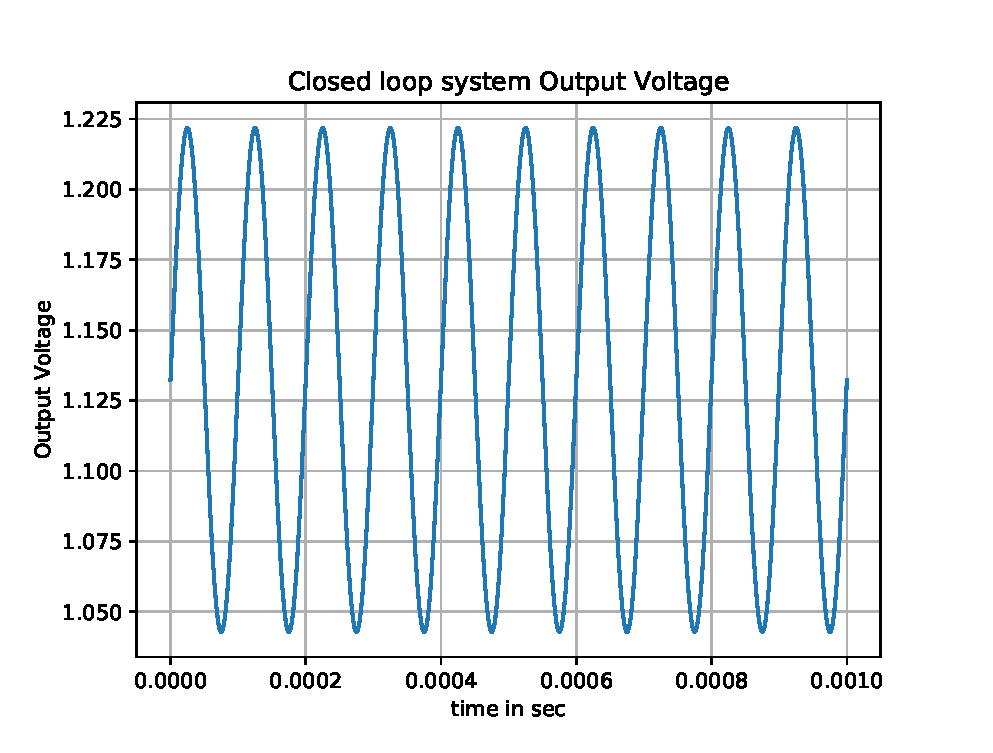
\includegraphics[width=\columnwidth]{./figs/ee18btech11046/ee18btech11046.eps}
\caption{Output Voltage}
\label{fig:ee18btech11046_spice}
\end{figure}
%

\begin{lstlisting}
codes/ee18btech11046/spice/ee18btech11046.py
\end{lstlisting}
We can observe that $V_{o}$ is sum of sine wave amplified by a factor of 89500 for small signal input and large signal output $V_{C}$ which is close to the calculated values.














\end{enumerate}
